\section{Déroulement du travail}

% Un titre de section aussi long est \textbf{fortement déconseillé} mais j'ai configuré le header pour qu'il le gère.

\subsection{Description de la mission}

\subsubsection{Le site web Répertoire Vert}
~\\

Ma mission concernait le site web du projet Répertoire Vert.
\\\\
Le Répertoire Vert est un outil de référencement et d’évaluation des produits et services verts proposés dans un rayon de 130 km autour d’un point de référence (ici Genève). 
Il permettra au «consomm’acteur» de trouver le meilleur produit/service «vert» en toute confiance et à un prix raisonnable, 
et à l’entreprise proposant un produit/service, d’avoir une meilleure visibilité, une reconnaissance active, et de vendre davantage.
\\\\

Le répertoire vert propose une répartition de l’activité économique « verte » en 28
secteurs principaux, comme Alimentation et Boisson, Green Building ou encore Santé et Bien-être.
\\\\
Il détermine 4 niveaux de référencement basés sur une triple évaluation :\\
• Celle de l’association gaea21\\
• Celle des professionnels de la branche d’activité concernée\\
• Celle du public (les consomm’acteurs)\\
\\
Ainsi, les entreprises peuvent se démarquer des produits « pseudo-verts » mis en vente sur le marché de manière abondante, et par conséquent, donner confiance , orienter et informer le consom’acteur de manière éthique.
Ce projet se décline en un site web et une application mobile.
\\\\

\begin{figure}[H]
    \centering
    
\includegraphics[width=8cm]{logo_repertoire_vert.png}
    \caption{Logo du Répertoire Vert}
\end{figure}

Le site s'adresse donc aux entreprises proposant des produits et/ou services verts, aux particuliers souhaitant trouver ces produits et services, 
mais aussi aux villes/régions qui peuvent voir les entreprises vertes disponibles sur leur territoire. Il se compose donc de 3 parties distinctes, 1 pour chaque cible.
Je me suis occupée principalement de la partie dédiée aux entreprises.
\\\\
\begin{figure}[H]
    \centering
    
\includegraphics[width=\textwidth]{homepage_entreprise.png}
    \caption{Page d'accueil entreprise}
\end{figure}


Sur le site, une entreprise doit pouvoir se connecter, ajouter des produits et/ou services, visualiser son profil et ses statistiques.
Plus largement, on pourra visualiser l'ensemble des entreprises inscrites dans la région, mais également en fonction des secteurs d'activité. Le site devra aussi être un site e-commerce permettant d'acheter des produits et services verts.

\subsubsection{Fonctionnalités à réaliser}
~\\
Les tâches à réaliser se définissaient petit à petit. En effet il est important dans l'association de savoir prendre des initiatives : 
on nous donne les instructions dans les grandes lignes, à nous de voir précisément les différentes tâches à réaliser pour atteindre l'objectif posé.
\\\\
Au niveau des fonctionnalités donc, je devais dans un premier temps m'occuper de la représentation des entreprises sur des cartes. 

La 1ère devait figurer sur le profil de l'entreprise avec un point la représentant sur cette carte.

La 2nde devait être plus générale en affichant toutes les entreprises inscrites sur le Répertoire vert. 
Elle devait faire l'objet d'un filtre comportant plusieurs critères pour les entreprises : catégorie, sous-catégorie, code postal, prix des produits/services vendus, etc\dots

\begin{figure}[H]
    \centering
    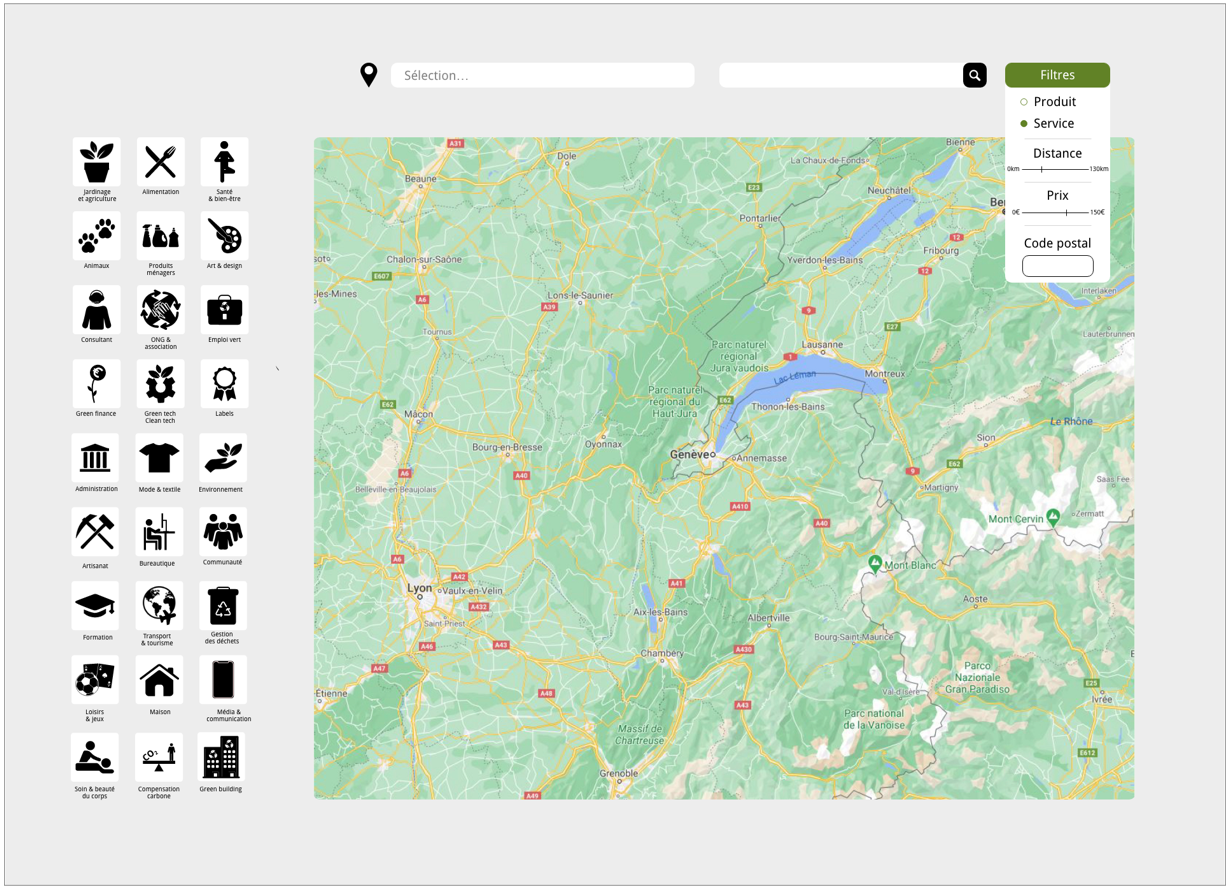
\includegraphics[width=\textwidth]{Carte.png}
    \caption{Design de la page carte à implémenter}
\end{figure}


Mais d'autres tâches se sont peu après avérées beaucoup plus urgentes que la carte des entreprises. J'ai donc dû me charger de rendre l'inscription, la connexion et la réinitialisation de mot de passe fonctionnelles, 
mais aussi de faire en sorte que l'utilisateur puisse visualiser et gérer entièrement son profil et ses produits/services. J'ai aussi travaillé sur le responsive du site et sur la création de diverses nouvelles pages. Toutes mes tâches seront détaillées dans la partie E.

\subsubsection{Gestion de projet}
~\\
Outre le développement web, mon autre rôle majeur était celui de chef de projet du Répertoire Vert, se constituant d'une équipe de 3 à 4 autres développeurs.
J'étais donc responsable du travail de mon équipe et devait m'assurer du respect des deadlines. Pour cela, il était parfois nécessaire de remplir des documents tels qu'un poker planning afin d'évaluer la difficulté des tâches et ainsi prévoir la durée de leur réalisation.
Cette responsabilité impliquait aussi la vérification du travail de mes coéquipiers, pour qu'il soit présentable au client et puisse être mis en production.
\begin{figure}[H]
    \centering
    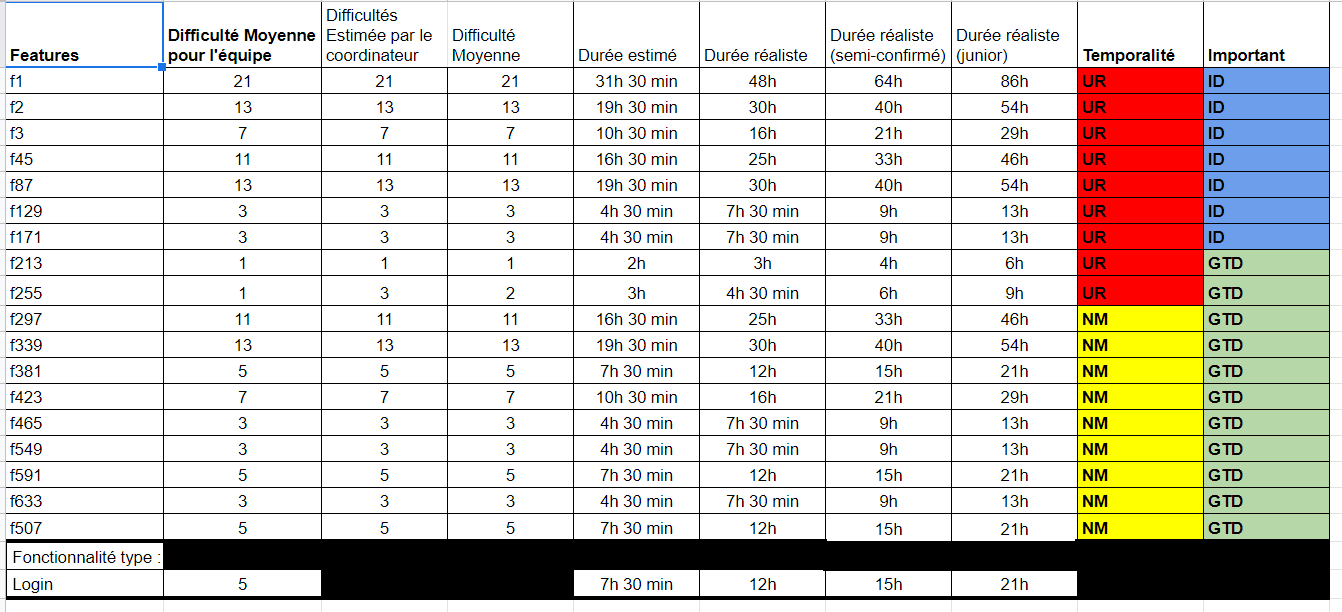
\includegraphics[width=\textwidth]{poker planning.png}
    \caption{Planning Poker}
\end{figure}

Être chef de projet signifiait également accueillir les nouveaux arrivants, en leur apportant toute l'aide dont ils ont besoin pour prendre en main le projet, notamment expliquer où se trouvent les différents fichiers, la méthodologie à adopter, ou encore les commandes utiles en invite de commandes. J'ai eu l'occasion d'accueillir 5 nouvelles recrues.
\\Mais même de manière plus générale, j'aidais souvent les membres de mon équipe dans leur tâche, ce qui m'a permis d'étudier des fonctionnalités sur lesquelles je n'étais normalement pas censée travailler.
\\\\
Tout cela m'a permis d'acquérir une vision globale du projet, me permettant de cerner les différentes tâches restantes et comment elles devaient être réalisées.
\\\\
Une autre responsabilité que j'avais était la mise en production du site web deux fois par semaine. 
\\Pour ce faire, il fallait mettre à jour le site sur un serveur Linux distant à l'aide de Git, un logiciel de gestion de versions que j'ai particulièrement utilisé durant ce stage. Cette étape de mise en production était très importante, car elle nous permettait d'appréhender d'éventuels bugs tout de suite plutôt que de les accumuler, ce qui assurait la qualité du rendu.


\pagebreak
\subsection{Antécédents}
~\\
Avant mon arrivée, le projet avait déjà été bien entamé, il a en effet débuté en Mars 2021, soit 5 mois auparavant. \\
- Une base de données était créée avec 59 tables, dont certaines remplies de données \\

\begin{figure}[H]
    \centering
    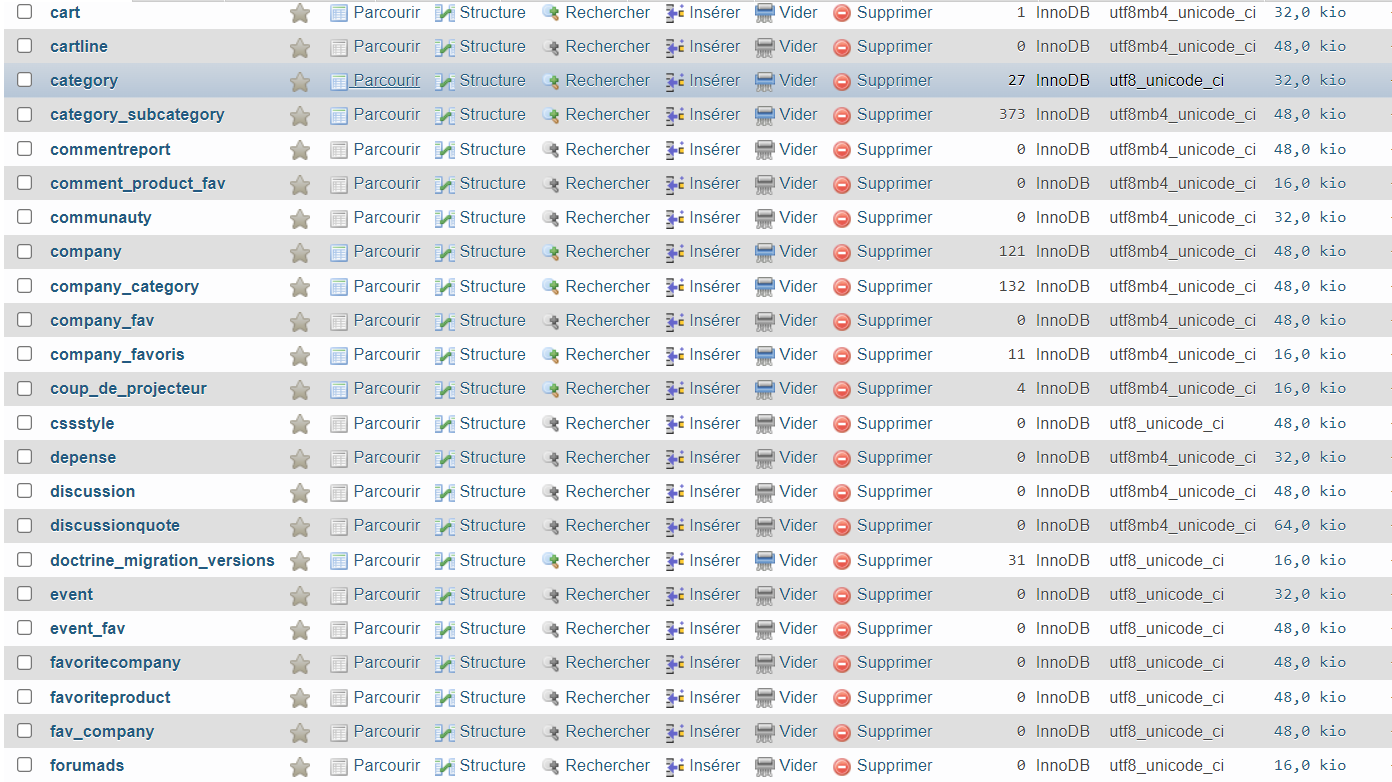
\includegraphics[width=\textwidth]{BDD.png}
    \caption{Extrait de la base de données du site Répertoire Vert}
\end{figure}

- De nombreuses pages avaient été intégrées conformément aux designs produits et validés \\

\begin{figure}[H]
    \centering
    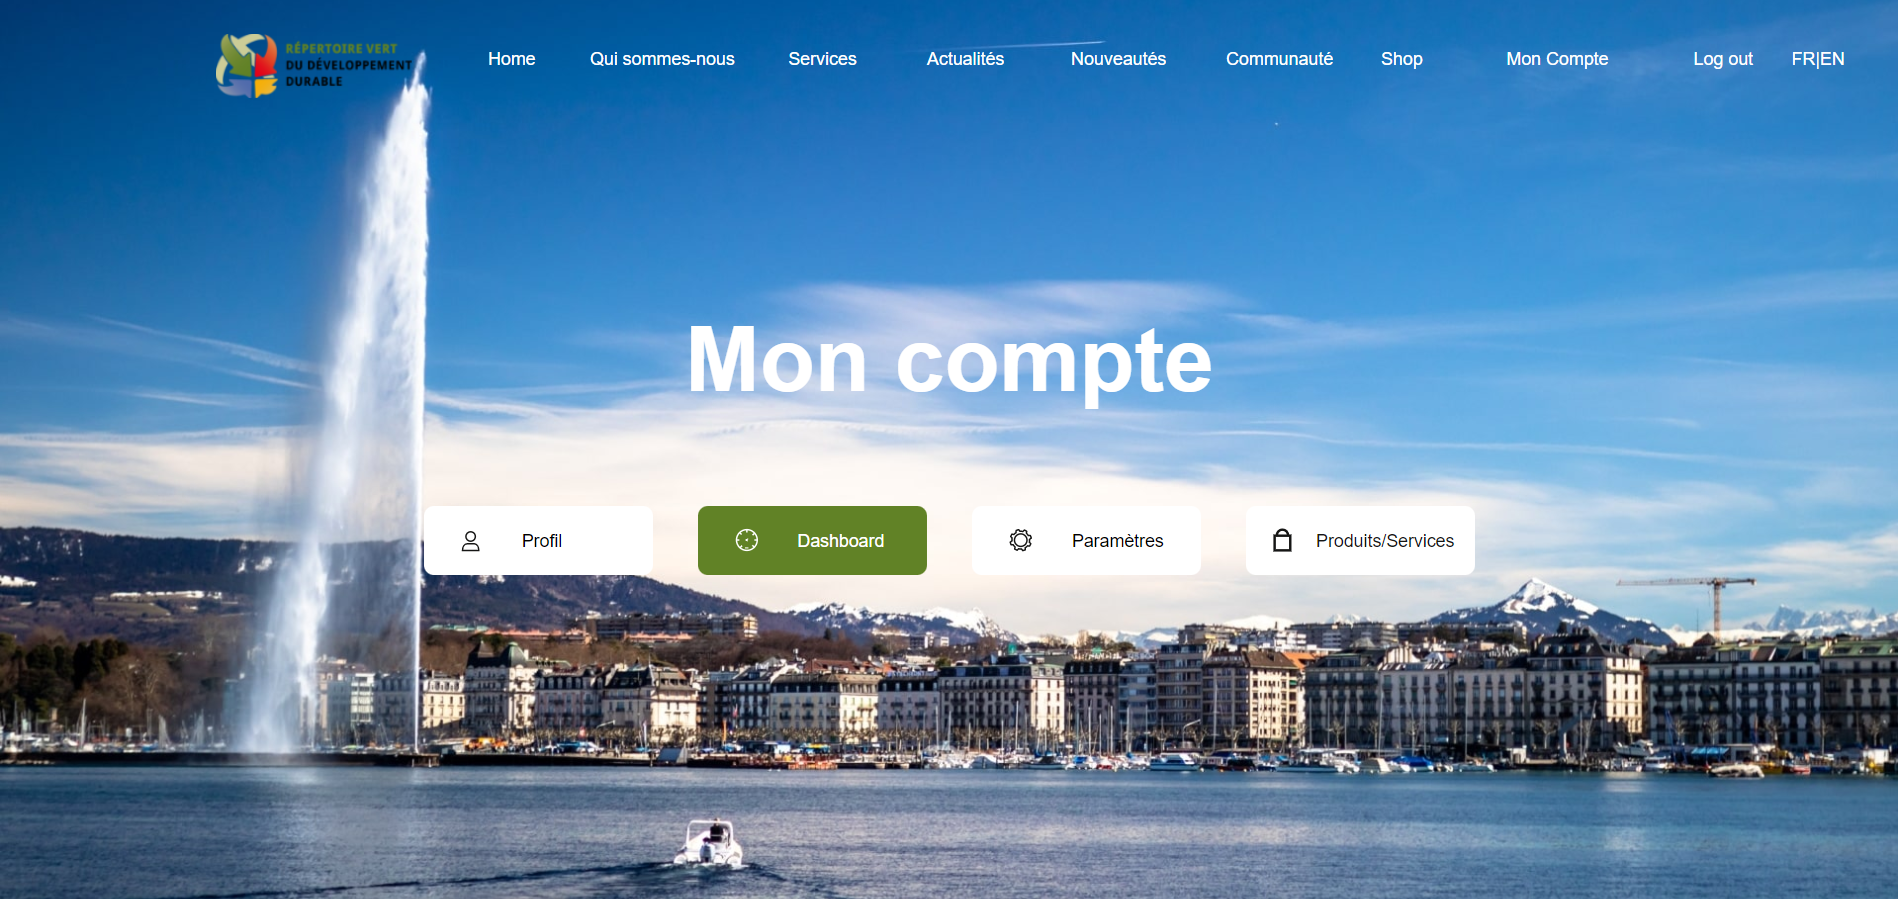
\includegraphics[width=\textwidth]{Header Dashboard.png}
    \caption{Exemple d'entête de page intégrée}
\end{figure}

- Certaines fonctionnalités avaient été implémentées partiellement ou complètement. Par exemple, l'inscription d'une entreprise était fonctionnelle à mon arrivée, mais certains champs ne l'étaient pas, comme l'upload d'un logo pour l'entreprise.
La plupart des pages intégrées n'étaient pas terminées, car les informations étaient entrées en dur, ou les fonctionnalités n'étaient pas abouties. \\

- Une API avait été créée par l'un des précédents membres de l'équipe et était utilisée pour tout ce qui concernait le compte d'un utilisateur, à savoir l'inscription, connexion, changement de mot de passe, etc... \\

\begin{callout}{Pourquoi une API ?}
Un compte sur le site du Répertoire Vert est transversal, c'est-à-dire qu'il peut être utilisé sur les autres sites créés par Gaea21. 
Par conséquent, les informations de connexion des utlisateurs sont stockées dans une autre base de données. 
Il fallait donc envoyer les données nécessaires à l'API via une requête Ajax ou PHP pour qu'un traitement soit fait dans la base de données distante. 
Cette API, dont voici la \href{https://gaea21user.sustlivprogram.org/swagger/#/}{documentation}, était donc déjà complètement fonctionnelle.
\end{callout}

Etant donné le turn-over important dans l'association, l'un des principaux défi était de se familiariser avec le code existant et les nombreux fichiers. 
Certaines fonctionnalités étaient déjà créées et pouvaient donc être réutilisées. Mais en parallèle, beaucoup de fichiers ou morceaux de code étaient inutilisés, et certains se répétaient. 
Il fallait donc savoir distinguer ce qui était utile de ce qui était à ignorer.

\pagebreak
\subsection{Objectifs visés et méthode choisie}

\subsubsection{Les objectifs}
~\\
Comme mentionné en partie II)A.2, les objectifs se définissaient au fil du stage. En effet, le grand objectif était l'avancement du site, mais les étapes n'étaient pas clairement définies dès le début du stage. 
J'ai listé l'ensemble des objectifs qui m'ont été donnés au fil des mois, il s'agit donc d'objectifs réalistes.\\\\

Avant toute chose, mon 1er objectif était l'accomplissement des formations STAFF 1 et STAFF 2 en 1 semaine, puis la formation ReactJS et Symfony en 3 semaines.
La formation Staff 1 concernait le développement durable et les projets de Gaea21, et la Staff 2 portait sur les outils Google très utilisés durant tout le stage.
\\\\A l'échelle de Gaea21, le 1er objectif était de livrer la version 0 du site. 
Cette version devait permettre à une entreprise de : 

\begin{itemize}
    \item S'inscrire et se connecter
    \item Visualiser son profil et modifier ses informations et son mot de passe
    \item Désactiver son compte
    \item Ajouter des produits et/ou services
    \item Visualiser ses produits/services, les supprimer et les modifier
    \item Visualiser ses statistiques, comme le nombre de clics sur ses produits
    \item Parcourir les différentes catégories et sous-catégories, et voir la liste des entreprises appartenant à chaque sous-catégorie.
    \item Visualiser les profils des autres entreprises ainsi que leurs produits/services
\end{itemize}

Cependant, je n'ai été au courant de cet objectif que 2 semaines après mon intégration au projet. 
Le 1er objectif que l'on m'avait donné pour le projet était celui des cartes mentionnées en partie A, qui devaient être prêtes pour la version 1. 

En effet, la version 0 était dejà censée être quasiment terminée à ce moment-là, c'est pourquoi on m'a attribué une tâche moins urgente. 
2 semaines plus tard, on m'a donc demandé d'aider un collègue à mettre en commun toutes les fonctionnalités pour mettre la V0 en production 
(autrement dit, merge toutes les branches Git sur la la branche principale).
C'est alors que nous nous sommes rendu compte que la V0 n'était pas du tout aboutie, c'est-à dire que presque aucune fonctionnalité de la liste ci-dessus n'était terminée. 
Or nous n'étions plus que 2 sur le projet. Il fallait donc basculer sur ces tâches en priorité.
\\\\
Une fois la V0 terminée en version ordinateur, L'objectif était de faire le responsive de toutes les pages intégrées. 
\\
En parallèle, pour le lancement du site, il fallait aussi ajouter à la base de données une soixantaine d'entreprises qui avaient dejà été inscrites, mais qui ont été supprimées durant le développement.
Elles devaient alors recevoir un mail afin de réinitialiser leur mot de passe.\\
\\\\
Pour finir, nous devions également entamer la page Actualités ainsi que l'inscription à la newsletter de Gaea21, à implémenter normalement pour la V1, mais qui ont été jugées finalement plus urgentes que le responsive de la V0.

\pagebreak

\subsubsection{La méthodologie}
~\\
Durant toute la durée du stage, il y avait un suivi régulier, permettant une gestion de projet selon la méthode agile.
\\\\
Ainsi, cela fonctionnait par cycles répétés : 
\\
Tous les jeudis, une réunion avec l'ensemble du département IT et le client (Yvan, le responsable de l'association) avait lieu afin de recueillir ses besoins pour le site.\\
Si nécessaire, un poker planning était réalisé pour répartir les tâches efficacement selon les difficultés et le temps prévu. 
\\Tous les jours, une réunion de suivi avec le tuteur et l'équipe permettait de partager notre avancée et obtenir de l'aide sur des points de blocage.
\\Pour finir, tous les lundi et jeudi, une mise en ligne du site était nécessaire pour garder la version en ligne toujours à jour et présentable au client.
\\\\En parallèle, il était très important de remplir les outils de suivi, à savoir : \\
- le journal de bord pour les heures et les tâches réalisées par jour/semaine/mois\\ 
- le tableau des tâches pour organiser les tâches à faire/en cours/faites, et répertorier le temps mis pour chacune d'entre elles.\\

Des points début, mi-stage et fin de stage étaient réalisés avec le tuteur et la coach RH pour vérifier le remplissage des outils et voir si tout allait bien.

\pagebreak
\subsection{Planning prévisionnel du travail}

\subsubsection{1er planning prévisionnel}
~\\

Les tâches étant ajoutées et révélées au fur et à mesure, il n'y avait pas de vision globale réaliste du projet en amont.\\
Le planning ci-dessous présente donc les prévisions ou souhaits d'Yvan et/ou de mes tuteurs au début de mon stage.\\ 
Mais comme toutes ces personnes travaillaient sur d'autres projets, elles n'étaient pas vraiment au courant de l'état d'avancement précis du projet, ce qui explique la grande différence entre ce planning et les objectifs listés précédemment.

\begin{figure}[H]
    \centering
    \includegraphics[width=\textwidth]{Planning prévisionnel.jpg}
    \caption{Planning prévisionnel}
\end{figure}

Il était donc prévu qu'après ma formation, je travaille sur la version 1 du site (en commençant par les cartes), 
pendant que le reste de l'équipe finalisait la V0. Je devais les aider également si besoin. Cette phase devait durer jusqu'aux vacances de Noël.
\\\\Pour information, la V1 devait contenir : \\
- Les pages "Qui sommes-nous", "Nouveautés", "Actualités" et "Communauté"\\
- La possibilité de noter des produits et entreprises, ainsi que de les mettre en favoris.
\\\\
Au retour des vacances, on ne m'a pas vraiment précisé ce que je ferais, mais les versions urgentes du Répertoire Vert devant être prêtes, on m'aurait sûrement mise sur un autre projet.
\\
La dernière semaine de stage était consacrée à la rédaction d'un rapport de transmission, permettant aux suivants de reprendre mon code.

\subsubsection{2nd planning prévisionnel}
~\\
Mi-septembre, le planning a pu évoluer en une version un peu plus réaliste.\\
Lorsque tout le monde a compris que la V0 n'était en réalité pas du tout terminée, Yvan nous avait fixé la deadline pour cette version au 7 octobre.
\\Après cela, il fallait rendre les pages fonctionnelles responsive. Et une fois cela terminé, nous pouvions nous atteler à la V1.

\begin{figure}[H]
    \centering
    \includegraphics[width=\textwidth]{Planning prévisionnel mi-stage.jpg}
    \caption{Planning prévisionnel de septembre}
\end{figure}

\pagebreak
\subsection{Application de la méthode}

\subsubsection{Formation React et Symfony}

Le 1er mois de stage était donc consacré à la formation ReactJS et Symfony 5.\\\\
J'ai commencé par ReactJS, en suivant un cours du site Graphikart sur ce framework. 
J'y ai appris les bases, ainsi que des notions plus avancées, comme les hooks, contextes, etc...
Des petits exercices faits par l'association m'ont permis de consolider mes acquis.\\\\

1 semaine après, j'ai débuté la formation Symfony, qui se faisait quant à elle sur le site SymfonyCasts, avec des vidéos également.
J'ai donc pu apprendre les bases de ce framweork, avec le principe de routes, services, bundles, contrôleurs, mais aussi la partie bases de données avec Doctrine.\\\\

La finalité de ces deux formations était un exercice dont l'objectif était de réaliser un CRUD (Create, Read, Update, Delete) liant Symfony et React.
Il était donc demandé :\\
\begin{itemize}
    \item D'afficher dans un tableau les informations d'une table "utilisateur" de la base de données avec ReactJS, après l'avoir créée.
    \item D'ajouter les fonctionnalités supprimer et modifier pour chaque ligne, et aussi ajouter un nouvel utilisateur.
    \item D'ajouter les possessions de l'utilisateur, visibles sur une autre page en cliquant sur le nom d'un utilisateur, et de pouvoir en ajouter.
    \item De calculer l'âge de l'utilisateur grâce à un service.
\end{itemize}

La 1ere chose à faire était la \textbf{création de l'entité Utilisateur} avec tous ses attributs, en ligne de commande.
\begin{figure}[H]
    
\includegraphics[width=6cm, left]{makeEntity.png}
\end{figure}


Puis, une fois la page créée grâce à un fichier \textbf{Twig} (front-end) et une fonction dans le \textbf{contrôleur} indiquant la route vers cette page (back-end), il fallait afficher les informations de la base de données dans un tableau html, en passant par \textbf{React}.\\
Pour ce faire, il fallait tout d'abord récupérer l'ensemble des informations de chaque utilisateur via le controleur. J'ai donc fait \textbf{une requete Doctrine} via le Repository de l'entité Utilisateur.
\\Puis, il fallait envoyer ces données au javascript sous forme de tableau json. Chaque page de l'application correspondait à un \textbf{composant React}. 
Le tableau affichant les utilisateurs était donc un composant récupérant les données dynamiquement par son état, via une \textbf{requête Ajax GET}.\\
Quant à la suppression d'un utilisateur, on appelle la fonction de suppression située dans le contrôleur Symfony via une \textbf{requête Ajax POST}.\\
Les fonctionnalités d'ajout et de modification reposent sur le même principe.\\
Pour calculer l'âge il suffisait d'importer le service en question dans le controleur afin d'utiliser la fonction.\\
Voici donc le résultat de ces 1eres fonctionnalités :

\begin{figure}[H]
    \centering
    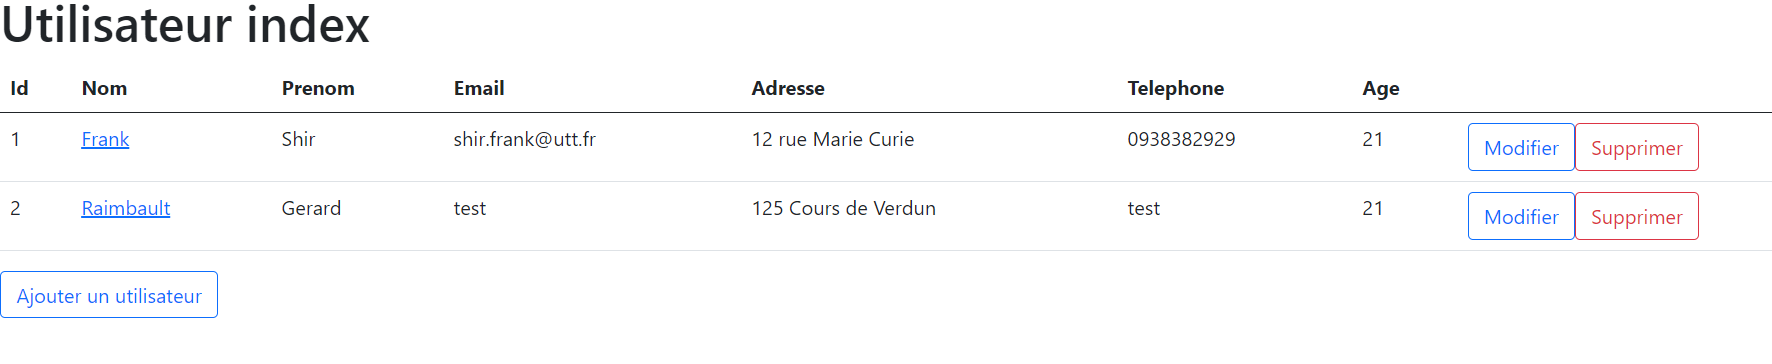
\includegraphics[width=\textwidth]{ExC_index.png}
    \caption{Accueil de l'appli}
\end{figure}

\begin{figure}[H]
    \centering
    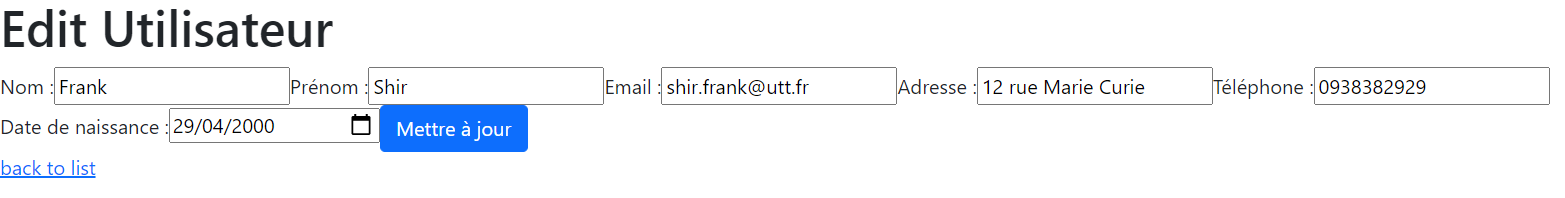
\includegraphics[width=\textwidth]{ExC_edit.png}
    \caption{Modification d'un utilisateur}
\end{figure}



Pour ajouter les possessions de chaque utilisateur, une nouvelle table/entité était nécessaire, ayant une relation \textbf{ManyToOne} du côté de la possession. 
Cela signifie qu'un utilisateur peut avoir plusieurs possessions, mais qu'une possession ne peut appartenir qu'à un seul utilisateur. \\
Il était facile de récupérer les possessions d'un utilisateur selon son id, mais la difficulté était la sérialisation des données à envoyer au JS sous forme de tableau json.
En effet, on récupérait un tableau de tableaux. Il fallait donc boucler dans le 1er tableau pour sérialiser chaque possession.\\
Une fois cela terminé, j'ai développé la fonctionnalité d'ajout d'une possession, comme pour les utilisateurs.

\begin{figure}[H]
    \centering
    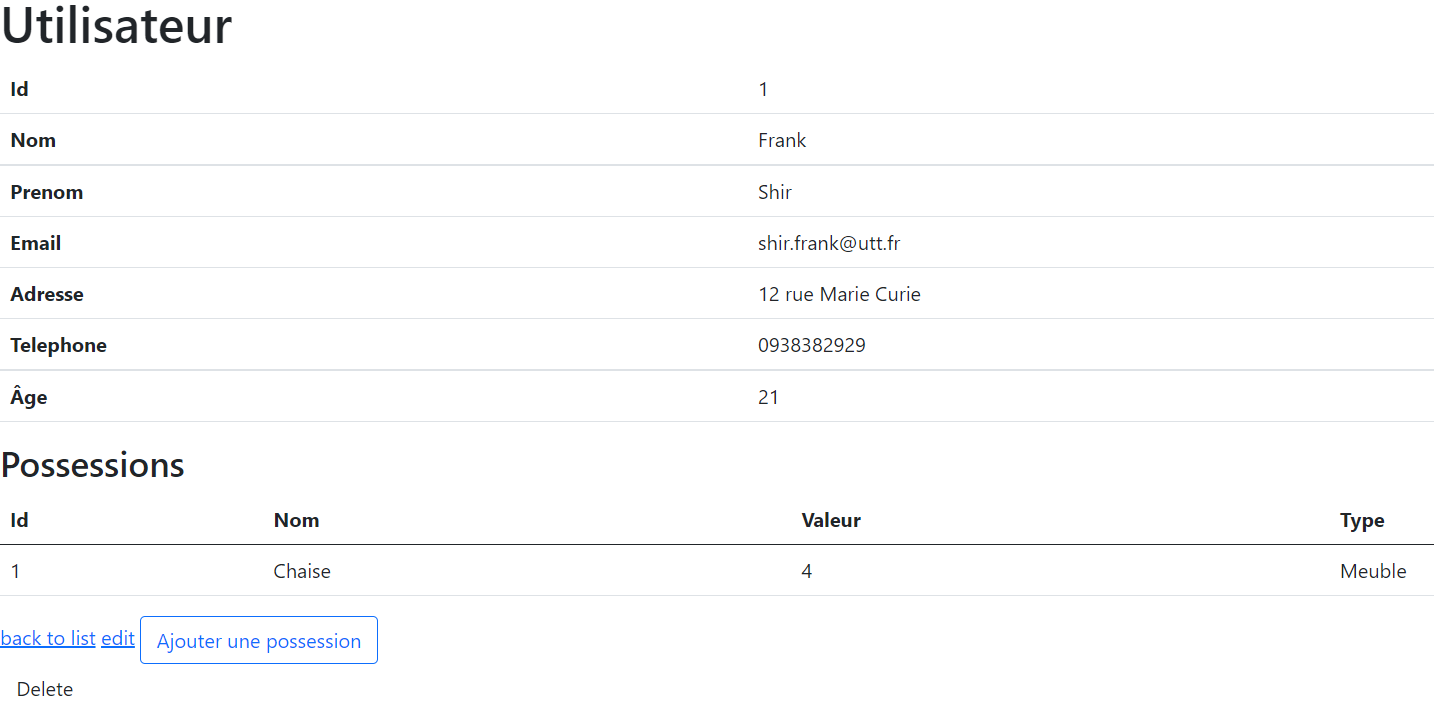
\includegraphics[width=\textwidth]{ExC_possessions.png}
    \caption{Page de l'utilisateur avec ses possessions}
\end{figure}

Une fois cet exercice validé, j'ai pu être intégrée au projet Répertoire Vert.


\subsubsection{Cartes des entreprises}

\paragraph{Carte d'1 entreprise}
Ma toute première tâche était donc l'intégration d'une carte permettant à l'entreprise de se localiser visuellement. Voici le design l'intégrant :

\begin{figure}[H]
    \centering
    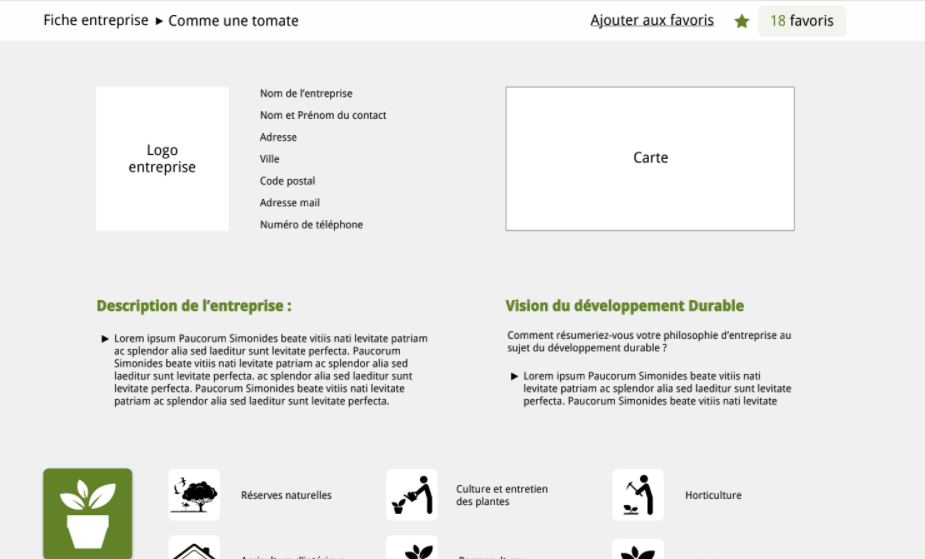
\includegraphics[width=\textwidth]{design_profil_carte.PNG}
    \caption{Design de la page profil avec la carte}
\end{figure}

Avant toute chose, j'ai étudié les différents fichiers existants, à la recherche d'un éventuel code que je pourrais réutiliser.
\\Il en existait effectivement un, une page avait été créée, contenant une carte avec toutes les entreprises de la base de données. \textbf{LeafletJS} était utilisée, une bibliothèque JavaScript libre de cartographie.
\\Il m'a simplement fallu modifier l'url de la requête ajax, afin de récupérer les coordonnées de non pas toutes les entreprises, mais d'une seule selon son id. J'ai également copié ce code dans un fichier javascript à part.

\begin{figure}[H]
    \centering
    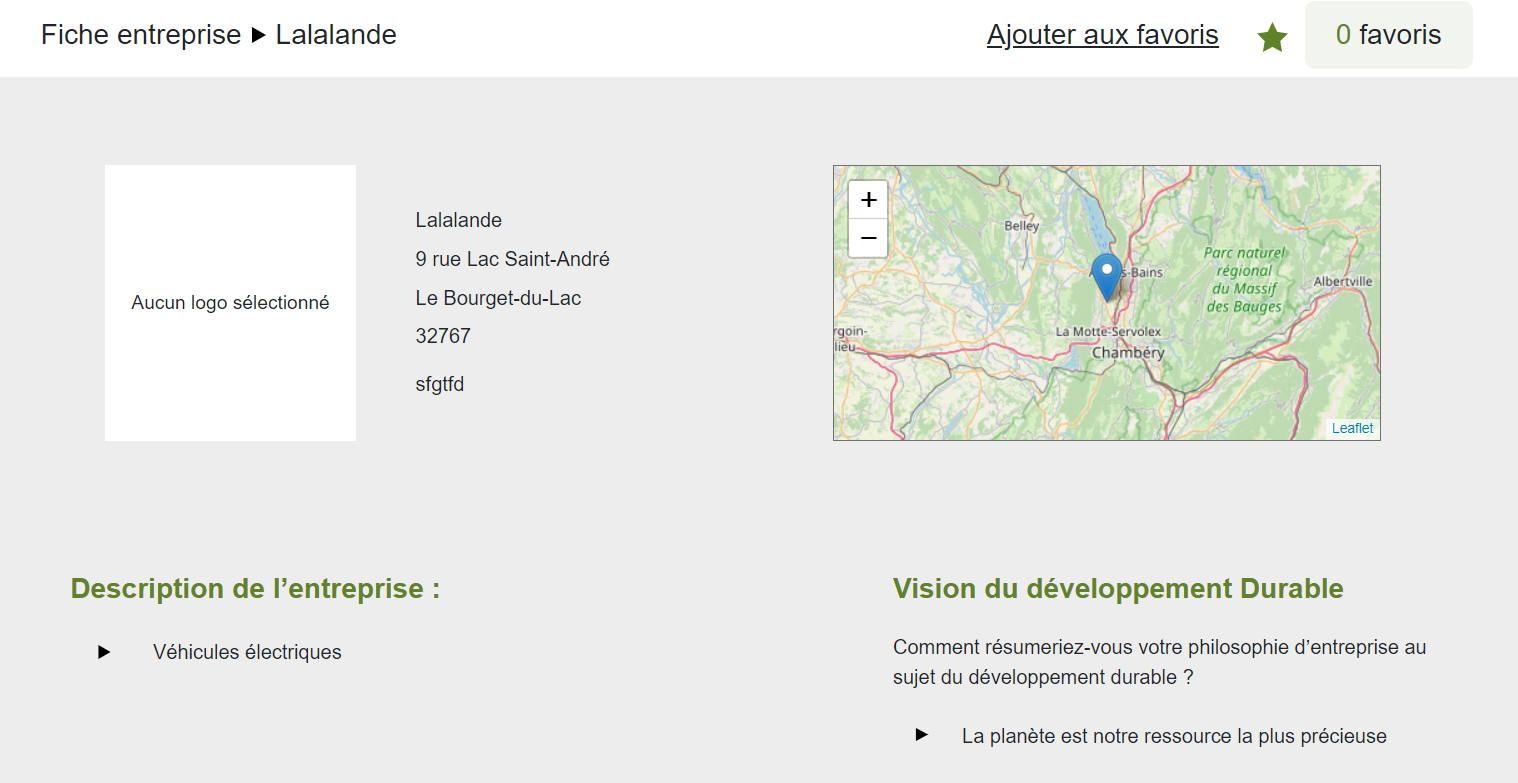
\includegraphics[width=\textwidth]{resultat_profil_carte.PNG}
    \caption{Résultat de la page profil avec la carte}
\end{figure}

Cependant, pour afficher l'emplacement de l'entreprise, il était nécessaire de récupérer les coordonnées GPS à partir de l'adresse, et ce dès l'inscription.\\
Après m'être familiarisée avec le code de l'inscription, j'y ai ajouté une requête Ajax vers l'API \textbf{OpenStreetMap} : "\emph{un projet collaboratif de cartographie en ligne qui vise à constituer une base de données géographiques libre du monde, en utilisant le système GPS et d'autres données libres}".
En mettant l'adresse en paramètre, on peut ainsi récupérer les latitude et longitude associées. Ces données sont ensuite envoyées au contrôleur pour être enregistrées en base de données.

\paragraph{Carte de toutes les entreprises}

La prochaine tâche concernait la page affichant toutes les entreprises sur une carte, avec la possibilité de les filtrer, et d'obtenir plus d'informations sur chaque entreprise :

\begin{figure}[H]
    \centering
    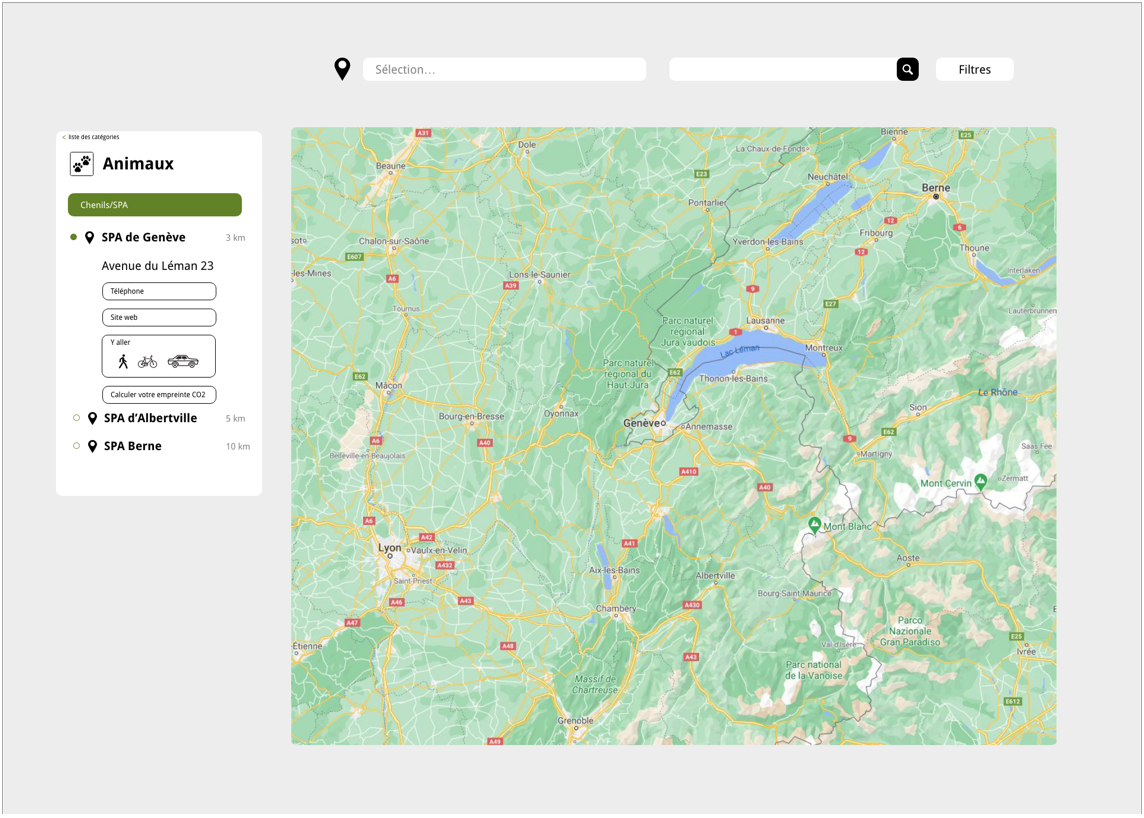
\includegraphics[width=\textwidth]{design_carte_details.PNG}
    \caption{Design page carte}
\end{figure}

J'ai décidé d'implémenter cette fonctionnalité en ReactJS, car l'affichage est considérablement modifié à chaque clic.
\\On a donc un composant principal qui est la carte, se chargeant d'afficher les bons points sur la carte et de les filtrer selon les critères reçus par les autres composants.
\\L'autre composant correspond au "Side Menu", qui s'affiche de 3 manières dans l'ordre ci-dessous.

\begin{figure}[H]
    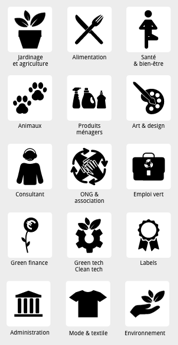
\includegraphics[width=5cm]{sidemenu1.PNG}
    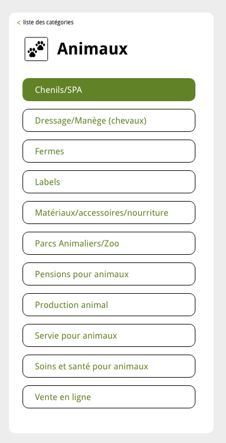
\includegraphics[width=5cm]{sidemenu2.PNG}
    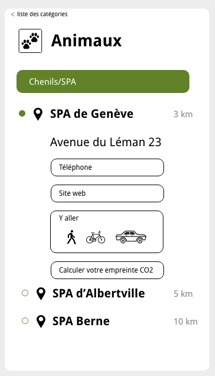
\includegraphics[width=5cm]{sidemenu3.PNG}
    \caption{Affichages successifs du side menu}
\end{figure}
On a d'abord les catégories, puis les sous-catégories, et enfin les entreprises correspondant à la sous-catégorie cliquée.

Récupération des entreprises appartenant à une sous-catégorie : ajout dans la table "product" d'un attribut company\_id car l'attribut initial "owner" renvoyait à un individu de l'entité "user".
Or un produit appartient forcément à une entreprise.
\\\\
Pb rencontré : Migrations de la bdd : DBB à jour mais pas le code => toutes les clées etrangeres sont deja créées ce qui crée des problèmes lors des migrations

\subsubsection{Rendre inscription et connexion fonctionnelles}

\subsubsection{Uploader une image}

\subsubsection{Ajouter - supprimer - modifier un produit ou service}

\subsubsection{Page profil et produits}

\subsubsection{Modification du profil}

\subsubsection{Nouvelles pages intégrées}
Tarifs/niveaux
Page en construction
Compte activé

\subsubsection{Carousel filtrant les produits}

\subsubsection{Activation manuelle des comptes}

\subsubsection{Tri des entreprises affichées sur la page sous-catégories}

\subsubsection{Ajout des entreprises manquantes}

\subsubsection{Réinitialisation de mot de passe}

\subsubsection{Rendre les graphes de statistiques du Dashboard fonctionnels}

\subsubsection{Responsive}
Pré-homepage\\
Homepage entreprise\\
Menu\\
Dashboard\\
Inscription


+ résolution bugs, front (comme désactivation compte, page sous categories)


Problèmes rencontrés
Git
Communication avec autres départements

\pagebreak
\subsection{Résultats par rapport à l'objectif et planning réel}

Parler du retard V0
\\De plus, ce projet était marqué par un fort turnover. Il fallait donc un temps d'adaptation et de familiarisation pour chaque nouvelle recrue, notamment pour l'installation du projet, savoir quel fichier correspondait à quoi, etc...
assigner des tâches qui correspondent aux objectifs de formation de chacun
Compétences acquises

% Une version humainement lisible d'une fork bombe peut s'écrire ainsi:
% % Il ny a pas de bashcode disponible
% \begin{minted}{bash}
% #!/bin/bash
% fbomb(){
%     fbomb | fbomb &
% }

% fbomb
% \end{minted}

% \subsubsection{Un plus gros bout de code !}
% \begin{listing}[H]
%     \inputminted{python}{src/parts/code/example.py}
%     \caption{square and multiply python code}
%     \label{cd:square_and_mult}
% \end{listing}

% \subsection{Une code sur plusieurs pages}

% \inputminted{python}{src/parts/code/example2.py}

% % https://tex.stackexchange.com/questions/12428/code-spanning-over-two-pages-with-minted-inside-listing-with-caption

% \subsection{Du code afficher plus simplement}

% Sinon, on peut directement utiliser le site \url{https://carbon.now.sh} ou en version raccourcie de l'url \shortUrl{https://carbon.now.sh} pour afficher du code en image ainsi :
% % Use H to place the figure HERE
% \begin{figure}[H]
%     \centering
%     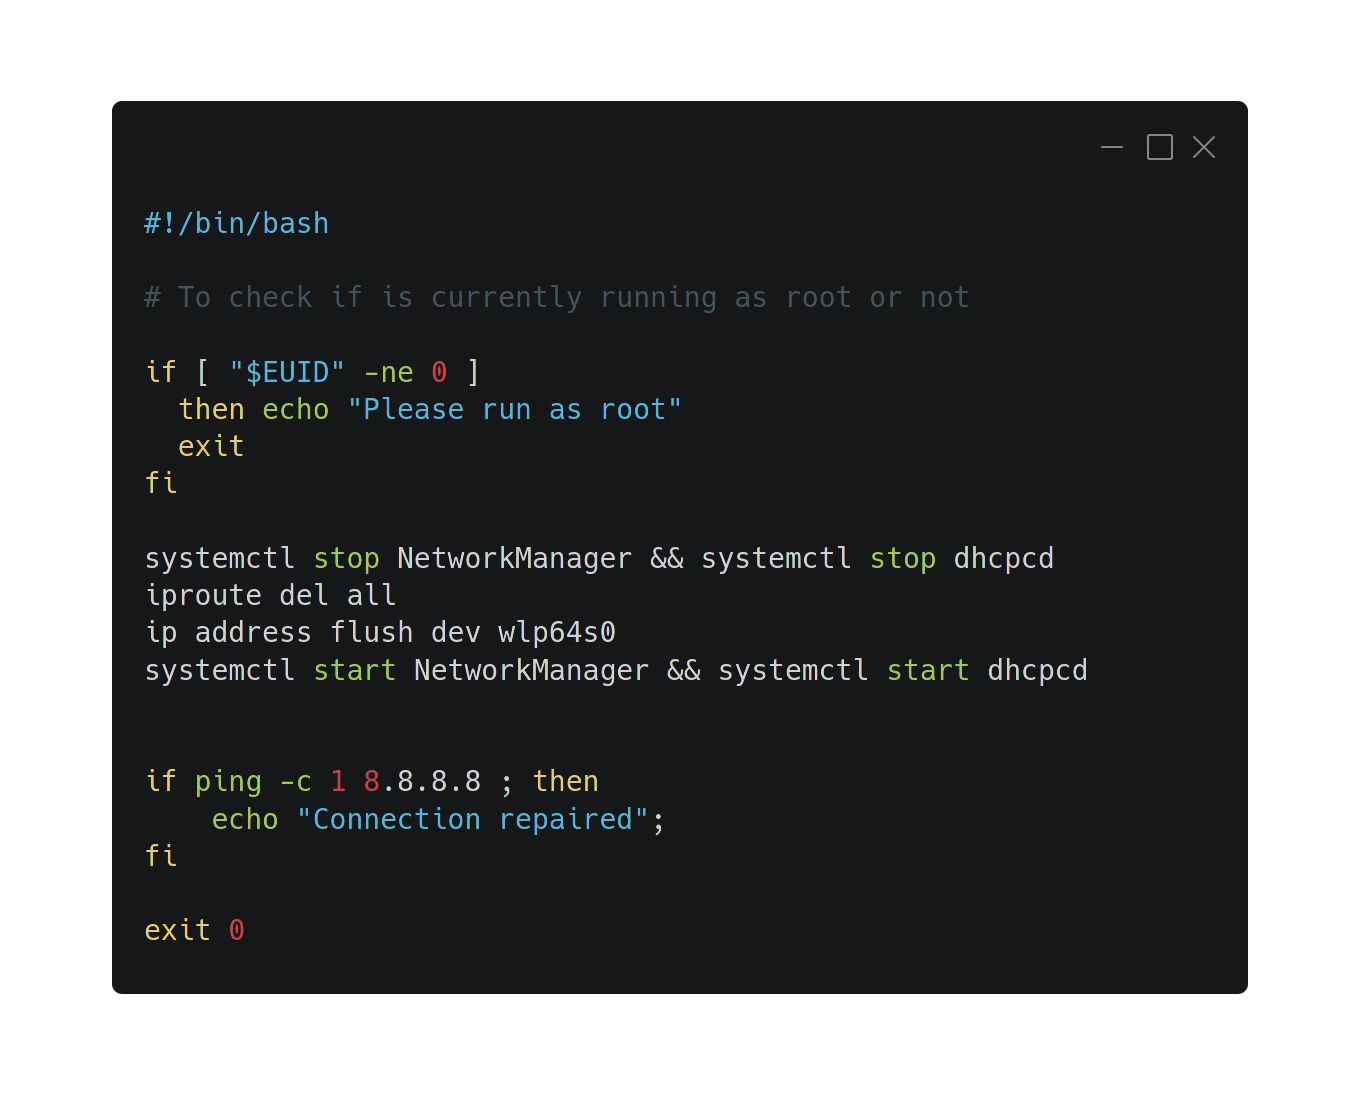
\includegraphics[width=\textwidth]{carbon.png}
% \end{figure}

% Gardez ce bout de code dans un coin, car ça m'a beaucoup aidé pour réparer automatiquement le
% "réseau" sur mon petit OS après qu'un méchant VPN mal configuré ait tout bazardé mes
% configurations.
% \ideaEnd
% On peut aussi afficher du "code" ou tout autre chose d'une façon "bloc note" avec ceci :
% \begin{mycodebox}
%     \begin{verbatim}
%         message :  Q     B     I     T
%         binary : 10000 00001 01000 10011
%         Key :    11100 01011 01001 10010
%         EncrB :  01100 00100 10010 00000
%         EncrM :    M     I     S     A
%     \end{verbatim}
% \end{mycodebox}

% Et si on a \yellowhl{envie} d'inclure directement un fichier \texttt{.txt}, on peut le faire !

% \VerbatimInput{src/contents/quCR_CHSH_Measurement.txt}

% On peut aussi choisir d'écrire directement du code au sein même de notre ligne. Si je veux expliquer que
% \incode{$x = y + 1$}, je peux.

